\subsection{Wood Texture Parameter Examples}
\label{appendix:wood-parameter-examples}

The following figures show exported examples of the Wood texture model. For each parameter, the left image shows the lowest tested value and the right image shows the highest tested value. All other parameters remain at the base configuration.

\begin{figure}[htbp]
    \centering
    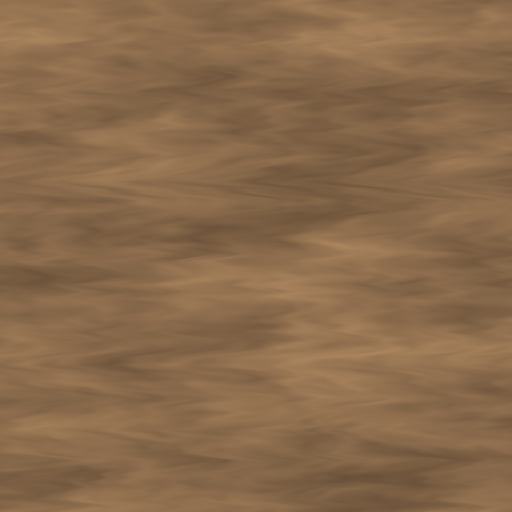
\includegraphics[width=0.35\textwidth]{figures/appendix/wood-param-control/wood-texture_base.png}
    \caption{Wood texture base configuration used as reference for the parameter comparisons.}
    \label{fig:wood-base}
\end{figure}

\begin{figure}[htbp]
    \centering
    \begin{tabular}{cc}
        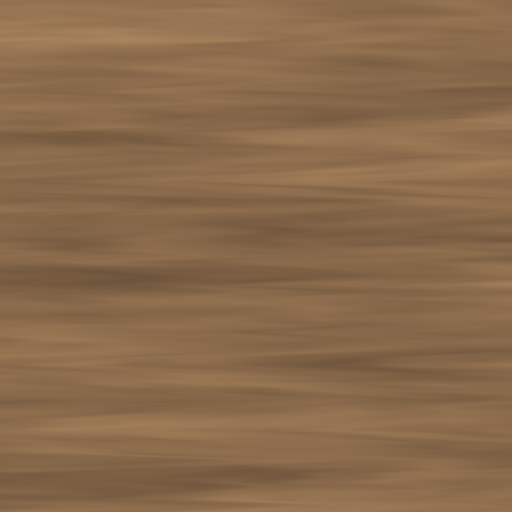
\includegraphics[width=0.45\textwidth]{figures/appendix/wood-param-control/wood-texture_anisotropy_0.10.png} &
        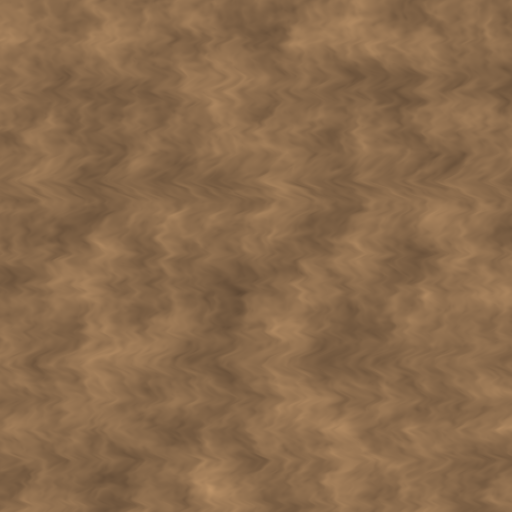
\includegraphics[width=0.45\textwidth]{figures/appendix/wood-param-control/wood-texture_anisotropy_1.00.png} \\[0.5em]
        Low value: 0.10 & High value: 1.00
    \end{tabular}
    \caption{Wood texture comparison for the anisotropy parameter. Lower values produce more directional stretching, while higher values reduce this directional compression.}
    \label{fig:wood-anisotropy}
\end{figure}

\begin{figure}[htbp]
    \centering
    \begin{tabular}{cc}
        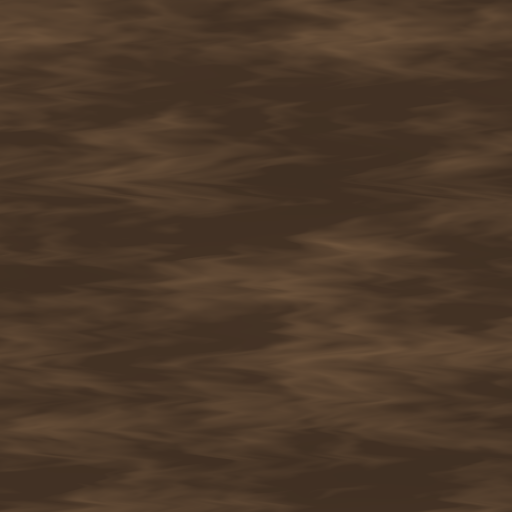
\includegraphics[width=0.45\textwidth]{figures/appendix/wood-param-control/wood-texture_brightness_-0.50.png} &
        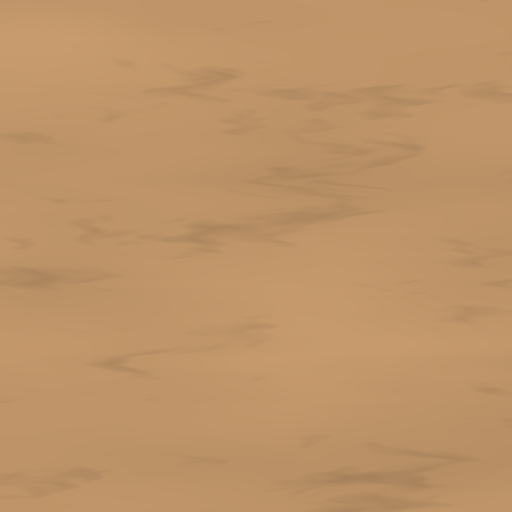
\includegraphics[width=0.45\textwidth]{figures/appendix/wood-param-control/wood-texture_brightness_0.50.png} \\[0.5em]
        Low value: -0.50 & High value: 0.50
    \end{tabular}
    \caption{Wood texture comparison for the brightness parameter. Lower values darken the generated texture, while higher values brighten the overall result.}
    \label{fig:wood-brightness}
\end{figure}

\begin{figure}[htbp]
    \centering
    \begin{tabular}{cc}
        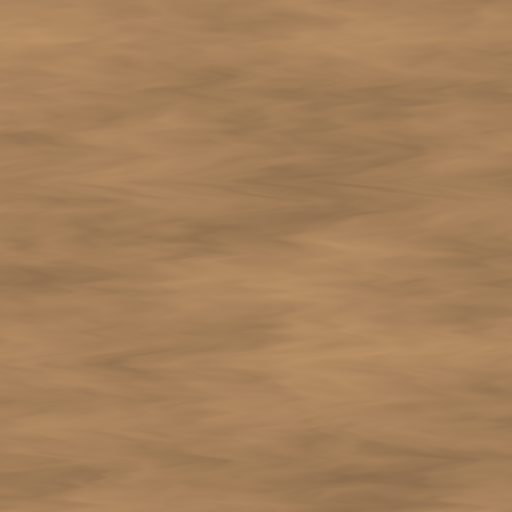
\includegraphics[width=0.45\textwidth]{figures/appendix/wood-param-control/wood-texture_contrast_0.50.png} &
        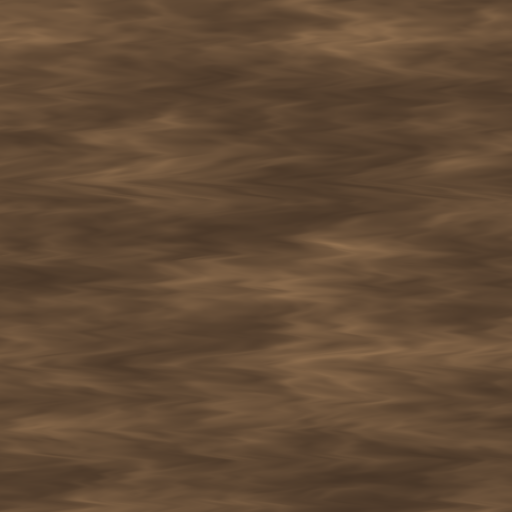
\includegraphics[width=0.45\textwidth]{figures/appendix/wood-param-control/wood-texture_contrast_3.00.png} \\[0.5em]
        Low value: 0.50 & High value: 3.00
    \end{tabular}
    \caption{Wood texture comparison for the contrast parameter. Lower values soften the difference between light and dark regions, while higher values make the grain pattern more pronounced.}
    \label{fig:wood-contrast}
\end{figure}

\begin{figure}[htbp]
    \centering
    \begin{tabular}{cc}
        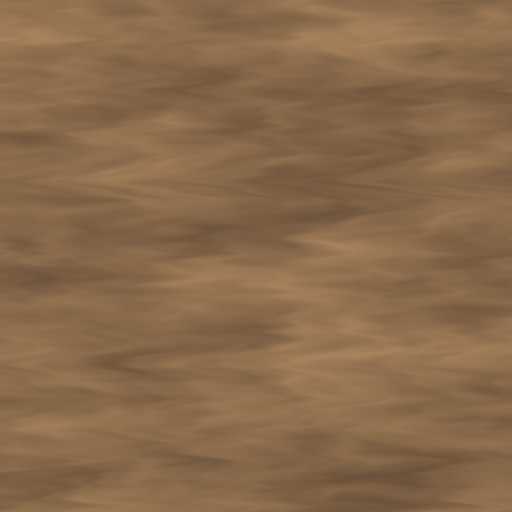
\includegraphics[width=0.45\textwidth]{figures/appendix/wood-param-control/wood-texture_crack_scale_2.00.png} &
        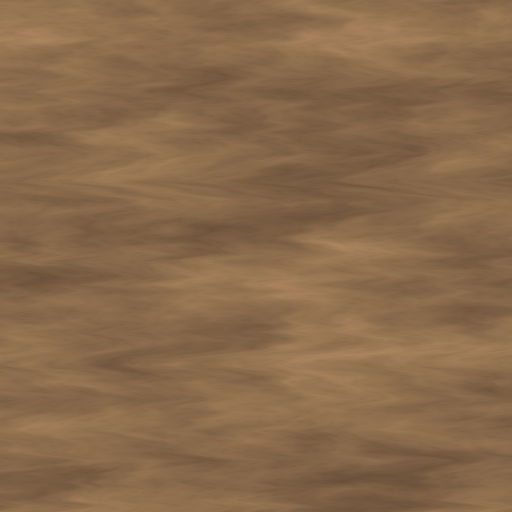
\includegraphics[width=0.45\textwidth]{figures/appendix/wood-param-control/wood-texture_crack_scale_15.00.png} \\[0.5em]
        Low value: 2.00 & High value: 15.00
    \end{tabular}
    \caption{Wood texture comparison for the crack scale parameter. Lower values create larger crack structures, while higher values create smaller and more frequent crack details.}
    \label{fig:wood-crack-scale}
\end{figure}

\begin{figure}[htbp]
    \centering
    \begin{tabular}{cc}
        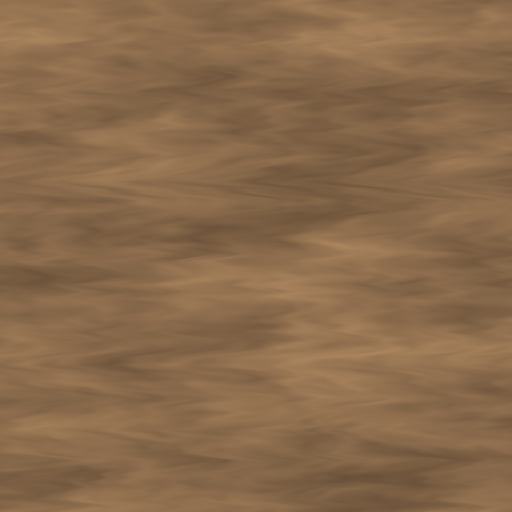
\includegraphics[width=0.45\textwidth]{figures/appendix/wood-param-control/wood-texture_crack_strength_0.00.png} &
        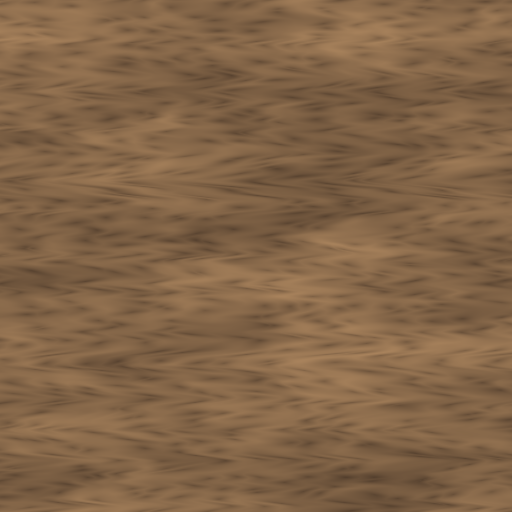
\includegraphics[width=0.45\textwidth]{figures/appendix/wood-param-control/wood-texture_crack_strength_0.50.png} \\[0.5em]
        Low value: 0.00 & High value: 0.50
    \end{tabular}
    \caption{Wood texture comparison for the crack strength parameter. Lower values remove crack influence, while higher values make crack-like structures more visible.}
    \label{fig:wood-crack-strength}
\end{figure}

\begin{figure}[htbp]
    \centering
    \begin{tabular}{cc}
        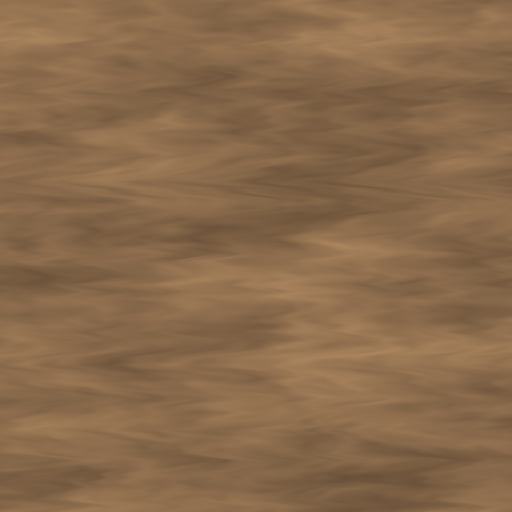
\includegraphics[width=0.45\textwidth]{figures/appendix/wood-param-control/wood-texture_detail_strength_0.00.png} &
        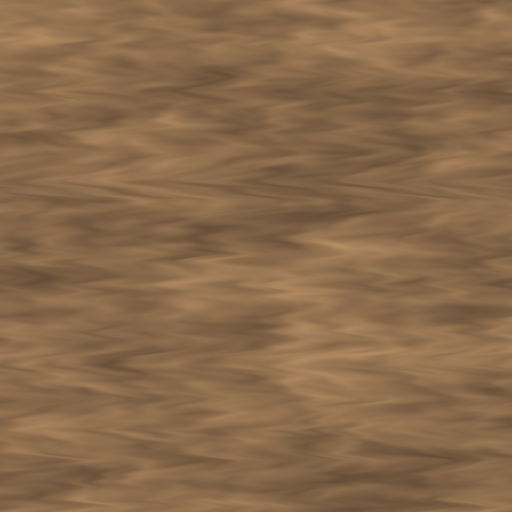
\includegraphics[width=0.45\textwidth]{figures/appendix/wood-param-control/wood-texture_detail_strength_0.50.png} \\[0.5em]
        Low value: 0.00 & High value: 0.50
    \end{tabular}
    \caption{Wood texture comparison for the detail strength parameter. Lower values reduce fine surface detail, while higher values add more small-scale variation to the grain.}
    \label{fig:wood-detail-strength}
\end{figure}

\begin{figure}[htbp]
    \centering
    \begin{tabular}{cc}
        
\includegraphics[width=0.45\textwidth]{figures/appendix/wood-param-control/wood-texture_grain_1.00.png} &
        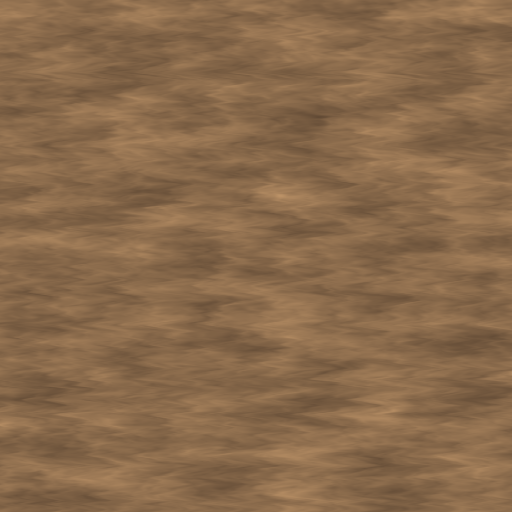
\includegraphics[width=0.45\textwidth]{figures/appendix/wood-param-control/wood-texture_grain_20.00.png} \\[0.5em]
        Low value: 1.00 & High value: 20.00
    \end{tabular}
    \caption{Wood texture comparison for the grain scale parameter. Lower values produce larger grain structures, while higher values produce finer and more frequent grain lines.}
    \label{fig:wood-grain}
\end{figure}

\begin{figure}[htbp]
    \centering
    \begin{tabular}{cc}
        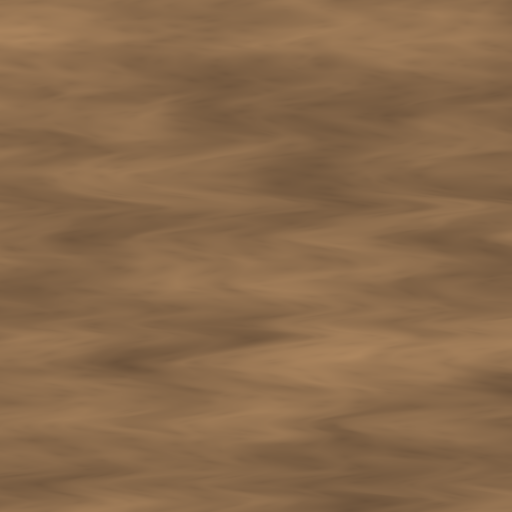
\includegraphics[width=0.45\textwidth]{figures/appendix/wood-param-control/wood-texture_Lacunarity_1.50.png} &
        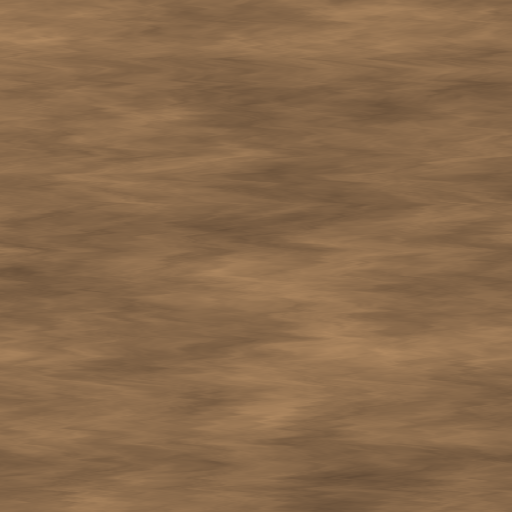
\includegraphics[width=0.45\textwidth]{figures/appendix/wood-param-control/wood-texture_Lacunarity_3.00.png} \\[0.5em]
        Low value: 1.50 & High value: 3.00
    \end{tabular}
    \caption{Wood texture comparison for the lacunarity parameter. Lower values keep octave frequencies closer together, while higher values increase frequency separation and create sharper multi-scale detail.}
    \label{fig:wood-lacunarity}
\end{figure}

\begin{figure}[htbp]
    \centering
    \begin{tabular}{cc}
        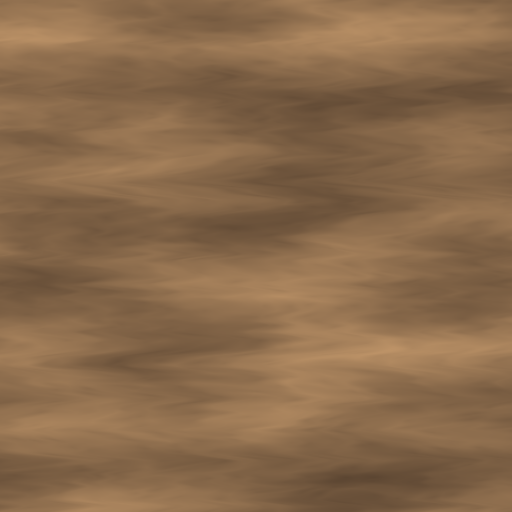
\includegraphics[width=0.45\textwidth]{figures/appendix/wood-param-control/wood-texture_octaves_1.png} &
        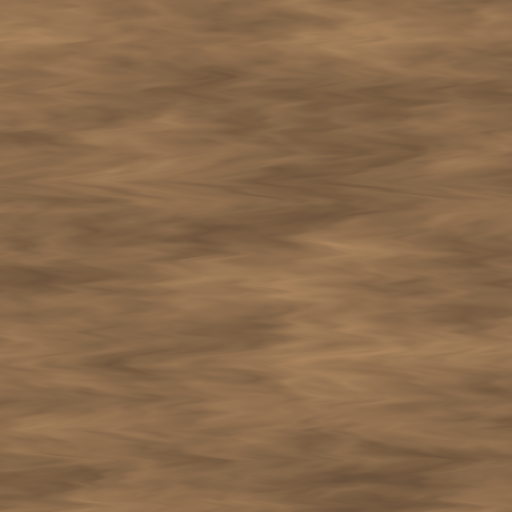
\includegraphics[width=0.45\textwidth]{figures/appendix/wood-param-control/wood-texture_octaves_6.png} \\[0.5em]
        Low value: 1 & High value: 6
    \end{tabular}
    \caption{Wood texture comparison for the octaves parameter. Lower values use fewer noise layers, while higher values add more layered detail to the texture.}
    \label{fig:wood-octaves}
\end{figure}

\begin{figure}[htbp]
    \centering
    \begin{tabular}{cc}
        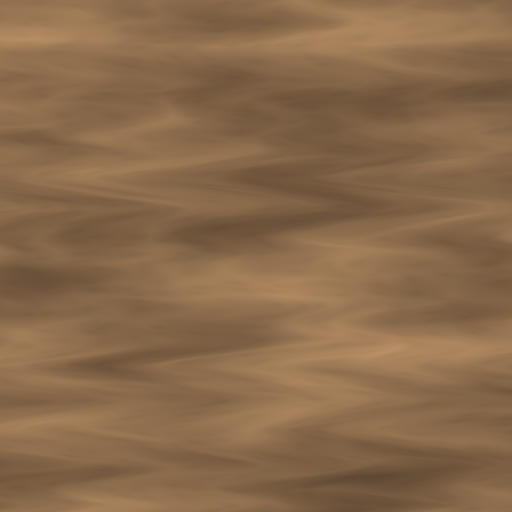
\includegraphics[width=0.45\textwidth]{figures/appendix/wood-param-control/wood-texture_persistence_0.10.png} &
        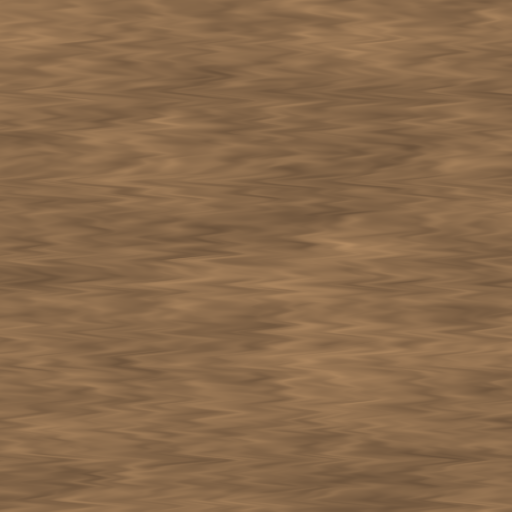
\includegraphics[width=0.45\textwidth]{figures/appendix/wood-param-control/wood-texture_persistence_0.90.png} \\[0.5em]
        Low value: 0.10 & High value: 0.90
    \end{tabular}
    \caption{Wood texture comparison for the persistence parameter. Lower values reduce the influence of higher-frequency layers, while higher values make fine details stronger.}
    \label{fig:wood-persistence}
\end{figure}

\begin{figure}[htbp]
    \centering
    \begin{tabular}{cc}
        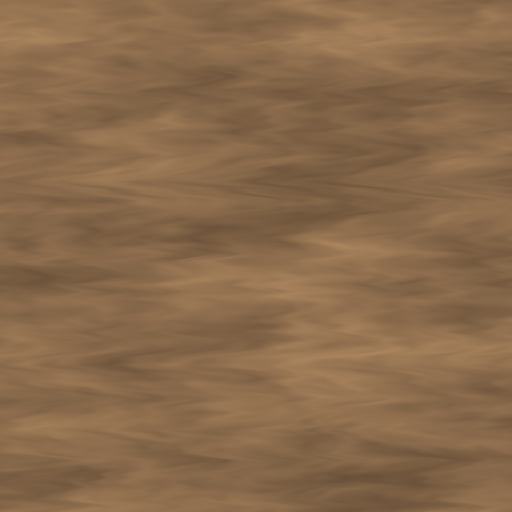
\includegraphics[width=0.45\textwidth]{figures/appendix/wood-param-control/wood-texture_ridge_strength_0.00.png} &
        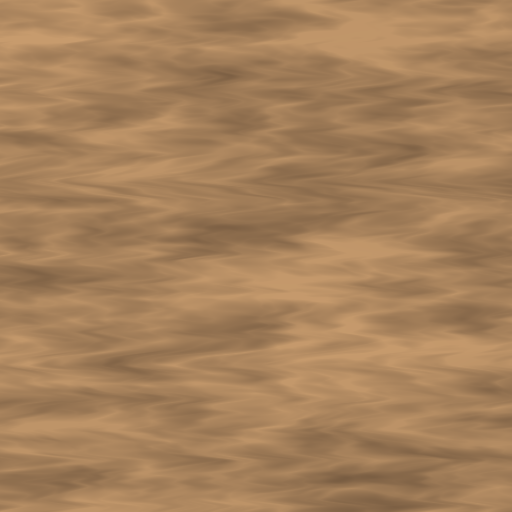
\includegraphics[width=0.45\textwidth]{figures/appendix/wood-param-control/wood-texture_ridge_strength_1.00.png} \\[0.5em]
        Low value: 0.00 & High value: 1.00
    \end{tabular}
    \caption{Wood texture comparison for the ridge strength parameter. Lower values reduce darker groove structures, while higher values emphasize ridges and grain boundaries.}
    \label{fig:wood-ridge-strength}
\end{figure}

\begin{figure}[htbp]
    \centering
    \begin{tabular}{cc}
        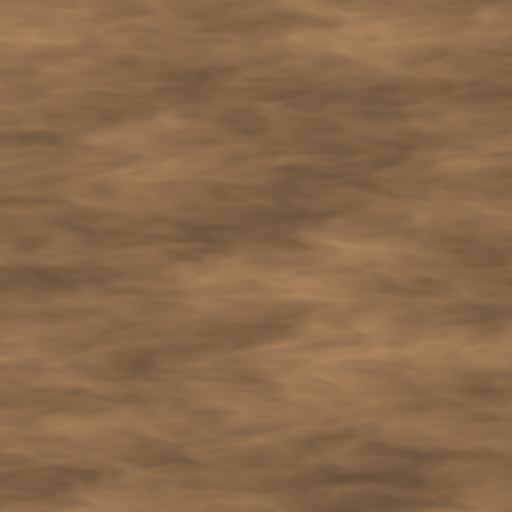
\includegraphics[width=0.45\textwidth]{figures/appendix/wood-param-control/wood-texture_warp_scale_0.50.png} &
        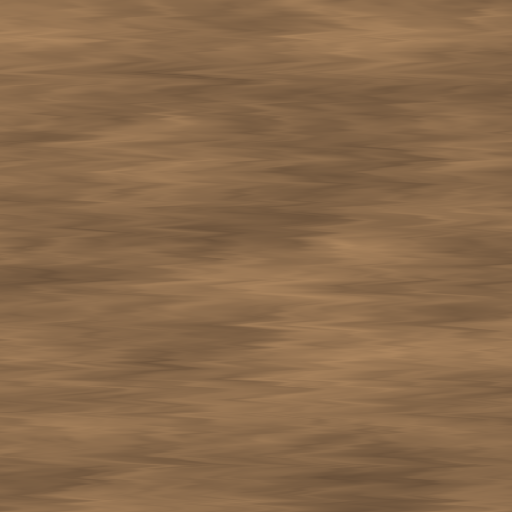
\includegraphics[width=0.45\textwidth]{figures/appendix/wood-param-control/wood-texture_warp_scale_5.00.png} \\[0.5em]
        Low value: 0.50 & High value: 5.00
    \end{tabular}
    \caption{Wood texture comparison for the warp scale parameter. Lower values create broad distortion waves, while higher values create more frequent local warping.}
    \label{fig:wood-warp-scale}
\end{figure}

\begin{figure}[htbp]
    \centering
    \begin{tabular}{cc}
        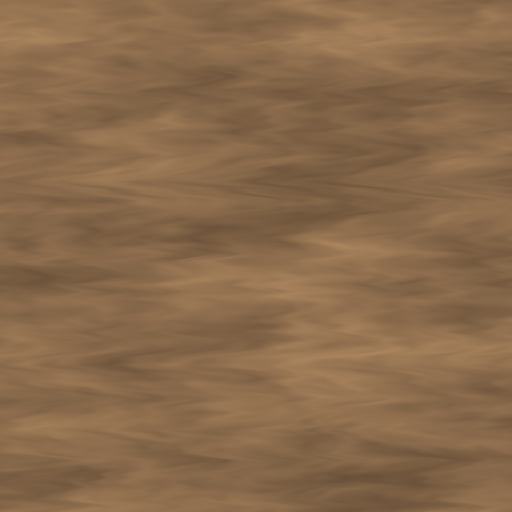
\includegraphics[width=0.45\textwidth]{figures/appendix/wood-param-control/wood-texture_warp_strength_0.00.png} &
        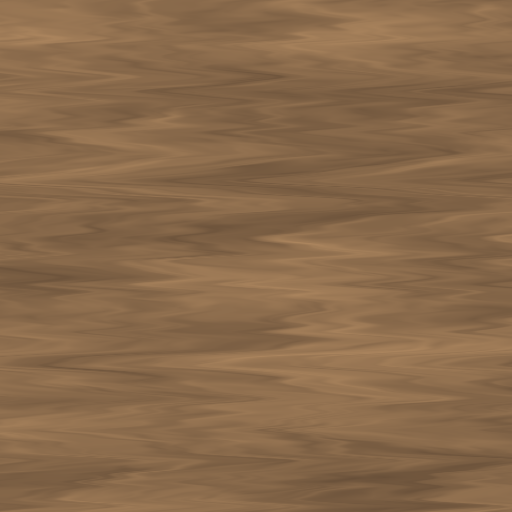
\includegraphics[width=0.45\textwidth]{figures/appendix/wood-param-control/wood-texture_warp_strength_2.00.png} \\[0.5em]
        Low value: 0.00 & High value: 2.00
    \end{tabular}
    \caption{Wood texture comparison for the warp strength parameter. Lower values keep the grain mostly regular, while higher values create stronger organic distortion.}
    \label{fig:wood-warp-strength}
\end{figure}